\appendix
\appendixpage
\addappheadtotoc
\section{Methods}

\subsection{Computational Environment}
We conducted the experiments on a machine with the following specifications:
\begin{itemize}
    \item Operating System: AlmaLinux release 8.9 ([core-4.1 kernel])

    \item  CPU:
    \begin{itemize}
        \item Architecture: x86\_64 (64-bit capable)
        \item Model: AMD Ryzen 9 3950X 16-Core Processor  
        \item Cores: 16 physical cores, 32 logical cores
        
    \end{itemize}
    \item Memory: 64\,GB total RAM
    \item Storage: NVMe device (KXG60PNV2T04 NVMe KIOXIA 2048\,GB)
\end{itemize}

7BGZF was compiled with clang (16.0.6). All other programs were compiled with gcc (8.5.0).



\subsection{Setting Compression Levels In SAMtools}\label{methodeComp}
In \sort, the user can set the compression level of the output file using the "\texttt{-l}" parameter. Possible options are integers from 0 to 9. Compression level 0 is equal to no compression (equal to the \texttt{-u} parameter).

For other SAMtools commands where the "\texttt{-l}" parameter does not exist, the user can still change the compression level of the output via adding \texttt{--output-fmt-option level=1} to the arguments of the command (Put the desired compression level between 0 and 9 instead of \texttt{1}).

\subsection{Configuring Libdeflate Support in HTSlib} \label{turnLibdeflate}

To decide manually between using zlib and libdeflate, the user can run the HTSlib \texttt{configure} script with the \texttt{--with-libdeflate} resp. \texttt{--without-libdeflate} option. To use \texttt{LD\_PRELOAD} for changing the zlib implementation, the user must build HTSlib without libdeflate.

\subsection{Libdeflate Compression Level Mapping}\label{compMapping}
\begin{table}[]
    \centering
    \begin{tabular}{l|>{\hspace{0.1em}} c >{\hspace{0.1em}} c >{\hspace{0.1em}} c >{\hspace{0.1em}} c >{\hspace{0.1em}} c >{\hspace{0.1em}} c >{\hspace{0.1em}}c >{\hspace{0.1em}} c >{\hspace{0.1em}} c}
         zlib & \hspace{0.1em} 1 & 2 & 3 & 4 & 5 & \textbf{6} & 7 & 8 & 9 \\
         libdeflate \hspace{0.1em} & \hspace{0.1em} 1 & 2 & 3 & 5 & 6 & \textbf{7} & 8 & 10 & 12 \\
    \end{tabular} \vspace{1em}
    \caption{Mapping between zlib compression levels and libdeflate compression levels in HTSlib. The default level is marked \textbf{bold}.}
    \label{tab:levelMapping}
\end{table}

\subsection{Configuring 7BGZF}\label{7bgzfConfig}

To configure the compression library and the compression level, 7BGZF uses to compress BAM files in the BGZF format, the user can set the \texttt{BGZF\_METHOD} environment variable to a compression library's name concatenated with a compression level before running a SAMtools command. 

For the compression libraries, users can choose one of {\texttt{zlib}}, {\texttt{miniz}}, {\texttt{slz}}, {\texttt{libdeflate}}, {\texttt{zlibng}}, {\texttt{igzip}}, and {\texttt{zopfli}}. Their possible compression levels vary:

\begin{itemize}
\itemsep 0mm
    \item {\texttt{zlib}}, {\texttt{miniz}}, and {\texttt{zlibng}} offer levels from \texttt{1} to \texttt{9}.
    \item {\texttt{libdeflate}} offers levels from \texttt{1} to \texttt{12}.
    \item {\texttt{igzip}} offers levels from \texttt{1} to \texttt{3}.
    \item {\texttt{slz}} only supports level \texttt{1}.
    \item While {\texttt{zopfli}} does not use compression levels in the traditional sense, it allows specifying an amount of iterations (greater than or equal to \texttt{1}) within the compression level parameter of 7BGZF.
\end{itemize}

Example for calling \sort with igzip and compression level 1: \\
\texttt{BGZF\_METHOD=igzip1 LD\_PRELOAD=/path/to/7bgzf.so samtools sort …}

\subsection{Using HTSlib as a Shared Library}\label{shared}

SAMtools uses HTSlib as static library by default. To override methods from HTSlib, SAMtools must use HTSlib as a shared library.
To use HTSlib as a shared library, the user has to change a single line in SAMtools' \texttt{config.mk.in} and change \texttt{@Hsource@HTSLIB = \$(HTSDIR)/libhts.a} to refer to \texttt{libhts.so} instead. Running SAMtools \texttt{./configure} script and \texttt{make} leads to SAMtools using HTSlib as a shared library. If SAMtools does not find the shared object, export the location of HTSlib in the \texttt{LD\_LIBRARY\_PATH} environment variable.


\subsection{Writing Uncompressed Temporary Files}\label{changeSource}

To remove the compression of temporary files, the source code of \sort must be changed.  
This can be done by replacing the parameter \texttt{mode} of the first call of \texttt{bam\_merge\_simple} in the \texttt{bam\_sort\_core\_ext} method, which is located in \texttt{bam\_sort.c}. Current values are, depending on the existence of a position too large to be stored in a BAM file, "\texttt{wzx1}" for BGZF compressed SAM files on compression level 1 and "\texttt{wbx1}" for BAM files with compression level 1. Those can be changed to "\texttt{w}" for SAM files and "\texttt{wbx0}" for uncompressed BAM files.

% \section{Profiling Timeline Screenshots}

% \begin{figure}
%     \makebox[\textwidth]{
%     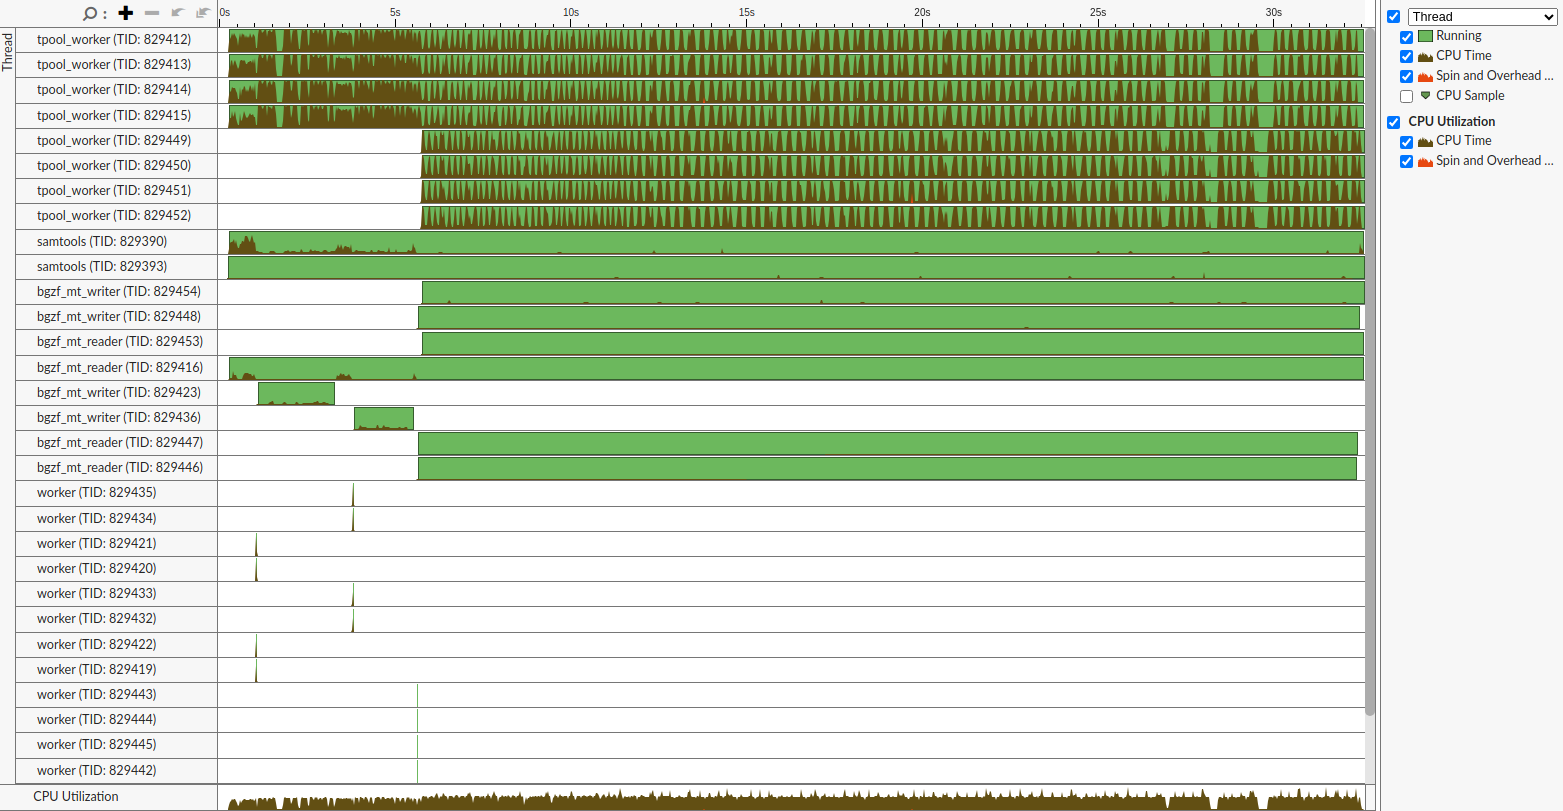
\includegraphics[width=1.5\linewidth]{figures/timelinePipe.png}}
% \caption{Screenshot of the VTune profiler on running \sort piped to SAMtools \texttt{view}. Both commands utilize 4 threads. However, the total of 8 CPUs the testing machine provides is never reached, as visualized under CPU Utilization. After 5.7 seconds, \sort starts merging the two temporary files it created before into the pipeline. The pipeline's buffer size is 1\,MB and the resulting file has a size of 230\,MB. In the merging and writing phase of \sort, 230 alternating spikes in CPU Time in the workers responsible for compression and decompression of \sort (first 4 rows) and SAMtools \texttt{view} can be found, indicating compression being a bottleneck of the piped operation.} \label{fig1}
% \end{figure}



\newpage